\documentclass[aspectratio=169,10pt]{beamer}

\usepackage[T1]{fontenc}
\usepackage{lmodern}

\usepackage{graphicx}
\usepackage{tikz}
\usetikzlibrary{positioning,arrows.meta}
\usepackage{xcolor}
\usepackage{booktabs}
\usepackage{tabularx}
\usepackage{array}
\usepackage{ragged2e}

% Typography & Box constraints
\setlength{\parskip}{0pt}
\setlength{\emergencystretch}{3.5em}
\hfuzz=2pt
\vfuzz=2pt
\setlength{\tabcolsep}{2.5pt}
\setlength{\leftmargini}{1.1em}
\setlength{\leftmarginii}{0.9em}

% Native Beamer compact list spacing
\def\tightlistspacing{%
  \setlength{\itemsep}{1.2pt}%
  \setlength{\parsep}{0pt}%
  \setlength{\topsep}{1pt}%
  \setlength{\partopsep}{0pt}%
}

\definecolor{GEUBlue}{RGB}{20,55,105}
\definecolor{GEULightBlue}{RGB}{238,244,251}
\definecolor{GEUGrey}{RGB}{90,90,90}
\definecolor{GEULightGrey}{RGB}{245,246,248}

\usetheme{default}
\setbeamertemplate{navigation symbols}{}
\setbeamertemplate{blocks}[rounded][shadow=false]
\setbeamercolor{normal text}{fg=black,bg=white}
\setbeamercolor{frametitle}{fg=GEUBlue}
\setbeamercolor{structure}{fg=GEUBlue}
\setbeamercolor{block title}{fg=GEUBlue,bg=GEULightBlue}
\setbeamercolor{block body}{fg=black,bg=GEULightBlue}
\setbeamerfont{frametitle}{size=\large,series=\bfseries}
\setbeamerfont{block title}{size=\footnotesize,series=\bfseries}
\setbeamerfont{block body}{size=\scriptsize}

% Fallback logo
\newcommand{\GEULogo}{%
  \IfFileExists{graphicera_logo.png}%
    {\includegraphics[height=0.48cm]{graphicera_logo.png}}%
    {\textcolor{GEUGrey}{\tiny Graphic Era}}%
}

% Clean headline and title rule
\setbeamertemplate{headline}{%
  \begin{tikzpicture}[remember picture,overlay]
    \node[anchor=north east,xshift=-0.35cm,yshift=-0.10cm]
      at (current page.north east) {\GEULogo};
  \end{tikzpicture}%
  \vspace{0.38cm}%
}

\setbeamertemplate{frametitle}{%
  \nointerlineskip
  \vspace{0.04cm}
  \insertframetitle\par
  \vspace{0.02cm}
  \textcolor{GEUBlue}{\rule{\textwidth}{0.8pt}}
  \vspace{0.04cm}
}

\setbeamertemplate{footline}{%
  \leavevmode
  \hbox{%
  \begin{beamercolorbox}[wd=.82\paperwidth,ht=0.28cm,dp=0.08cm,leftskip=.3cm]{author in head/foot}
    \tiny Department of Computer Science \& Engineering | Graphic Era (Deemed to be University)
  \end{beamercolorbox}%
  \begin{beamercolorbox}[wd=.18\paperwidth,ht=0.28cm,dp=0.08cm,rightskip=.3cm]{date in head/foot}
    \hfill\tiny\insertframenumber/\inserttotalframenumber
  \end{beamercolorbox}}%
}

% Hyperref-safe title and authors
\title[Project-Based Learning -- Phase-I Evaluation]{\texorpdfstring{\textbf{Project-Based Learning}\\[2mm]\large Phase-I Evaluation}{Project-Based Learning -- Phase-I Evaluation}}
\author[VERI NEWS (DSCPP-III-2026-T224)]{\texorpdfstring{\textbf{VERI NEWS}\\Team ID: DSCPP-III-2026-T224}{VERI NEWS -- Team ID: DSCPP-III-2026-T224}}
\institute[Graphic Era (Deemed to be University)]{\texorpdfstring{Department of Computer Science \& Engineering\\Graphic Era (Deemed to be University), Dehradun}{Department of Computer Science & Engineering, Graphic Era (Deemed to be University), Dehradun}}
\date[2026--27]{Academic Session 2026--27}

\begin{document}

% ============================================================
% 1. TITLE SLIDE
% ============================================================
\begin{frame}[plain]
\begin{tikzpicture}[remember picture,overlay]
\draw[GEUBlue,line width=3pt] (current page.north west) -- (current page.north east);
\node[anchor=north east,xshift=-0.45cm,yshift=-0.35cm] at (current page.north east)
  {\IfFileExists{graphicera_logo.png}{\includegraphics[height=1.0cm]{graphicera_logo.png}}{\textcolor{GEUGrey}{\bfseries Graphic Era}}};
\node[align=center,text width=.84\paperwidth] at ([yshift=.25cm]current page.center)
{
  {\color{GEUBlue}\fontsize{22}{26}\selectfont\bfseries PROJECT-BASED LEARNING}\\[2.5mm]
  {\fontsize{15}{18}\selectfont PHASE-I EVALUATION}\\[6mm]
  {\color{GEUGrey}\Large\bfseries VERI NEWS}\\[2.5mm]
  {\color{GEUBlue}\small Team ID: DSCPP-III-2026-T224}
};
\node[align=center,anchor=south,yshift=.38cm] at (current page.south)
{
  \footnotesize\bfseries Department of Computer Science \& Engineering\\
  Graphic Era (Deemed to be University), Dehradun\\[-0.5mm]
  \tiny Academic Session 2026--27
};
\end{tikzpicture}
\end{frame}

% ============================================================
% 2. TEAM AND MENTOR DETAILS
% ============================================================
\begin{frame}{Team \& Mentor Details}
\begin{columns}[T,totalwidth=\textwidth]
\column{.48\textwidth}
\begin{block}{Team Information}
\scriptsize
\begin{tabular}{@{}ll@{}}
\textbf{Team ID:} & DSCPP-III-T224\\
\textbf{Semester:} & 3rd\\
\textbf{Section:} & D, J, ML2\\
\textbf{Domain:} & Data Structures + OOP / C++
\end{tabular}
\end{block}

\column{.48\textwidth}
\begin{block}{Team Members}
\scriptsize
1.\quad Shambhavi Srivastava -- 2510012471\\[2pt]
2.\quad Abhinav Panwar -- 2512510050\\[2pt]
3.\quad Akshat Sharma -- 2510010700
\end{block}
\end{columns}

\vspace{3mm}
\begin{block}{Mentor}
\scriptsize
\textbf{Mentor Name:} Mr. Kamal Kumar Gola
\hfill
\textbf{Interactions completed:} \underline{\hspace{15mm}}
\end{block}
\end{frame}

% ============================================================
% 3. PROBLEM STATEMENT AND MOTIVATION
% ============================================================
\begin{frame}{Problem Statement \& Motivation}
\begin{block}{Problem Statement}
\scriptsize\RaggedRight
Online information can spread fast, making it hard for a user to determine what news is reliable and what is simply fake or suspicious.
Manual verification can be tedious and error-prone.
\end{block}

\vspace{1.5mm}
\begin{columns}[T,totalwidth=\textwidth]
\column{.48\textwidth}
\textbf{\color{GEUBlue}\footnotesize Motivation}
\begin{itemize}\scriptsize\tightlistspacing
\item Rapid spread of unverified information
\item Difficulty of checking every claim manually
\item Need for a simple preliminary verification tool
\item Need to compare claims with stored evidence
\end{itemize}

\column{.48\textwidth}
\textbf{\color{GEUBlue}\footnotesize Target Users / Stakeholders}
\begin{itemize}\scriptsize\tightlistspacing
\item General internet users
\item Students and researchers
\item News readers
\item Content moderators
\end{itemize}
\end{columns}
\end{frame}

% ============================================================
% 4. OBJECTIVES
% ============================================================
\begin{frame}{Objectives}
\textbf{\color{GEUBlue}\footnotesize Project Objectives}
\vspace{1mm}
\begin{enumerate}\small\tightlistspacing
\item Develop a solution for preliminary news verification.
\item Store and manage verified and suspicious news records.
\item Use DSA for efficient searching, indexing and matching.
\item Apply C++ OOP for modular application design.
\item Generate an explainable credibility / matching score.
\item Evaluate the system with predefined test cases.
\end{enumerate}

\vspace{2.5mm}
\begingroup
\centering
\noindent\colorbox{GEULightBlue}{%
\parbox{\dimexpr.88\textwidth-2\fboxsep\relax}{%
\centering\footnotesize
\textbf{Key Objective:} Provide users with a quick, explainable preliminary assessment of a news claim based on stored records and matching evidence.
}}%
\par
\endgroup
\end{frame}

% ============================================================
% 5. PROPOSED SOLUTION
% ============================================================
\begin{frame}{Proposed Solution}
\begin{block}{System Idea}
\scriptsize\RaggedRight
The system checks a news claim by extracting keywords, finding related stored records, and giving a preliminary result.
\end{block}

\vspace{1.5mm}
\begin{columns}[T,totalwidth=\textwidth]
\column{.48\textwidth}
\begin{block}{Main Features}
\begin{itemize}\scriptsize\tightlistspacing
\item News verification \quad $\bullet$ Keyword search
\item Similar-news detection \quad $\bullet$ Source checking
\item Verification report
\end{itemize}
\end{block}

\vspace{1mm}
\begin{block}{Input}
\begin{itemize}\scriptsize\tightlistspacing
\item Headline or news text
\item Existing news records
\end{itemize}
\end{block}

\column{.48\textwidth}
\begin{block}{Processing}
\begin{enumerate}\scriptsize\tightlistspacing
\item Extract keywords $\rightarrow$ Hash for lookup
\item Find related news $\rightarrow$ Search \& rank
\item Calculate matching score
\end{enumerate}
\end{block}

\vspace{1mm}
\begin{block}{Result}
\begin{itemize}\scriptsize\tightlistspacing
\item Likely Verified \quad $\bullet$ Needs Verification \quad $\bullet$ Suspicious
\end{itemize}
\end{block}
\end{columns}

\vspace{1.5mm}
\centering\tiny\textbf{Stored:} News records \;|\; Sources \;|\; Status \;|\; Search history
\end{frame}

% ============================================================
% 6. INTEGRATION OF PBL COURSE CONCEPTS
% ============================================================
\begin{frame}{Integration of PBL Course Concepts}
\begin{block}{PBL Integration}
\scriptsize\RaggedRight
DSA provides efficient storage and searching, while C++ OOP organizes the system into reusable classes and modules.
\end{block}

\vspace{1.5mm}
\begin{center}
\renewcommand{\arraystretch}{1.1}
\scriptsize
\begin{tabularx}{\textwidth}{@{}>{\bfseries\RaggedRight}p{2.3cm}>{\RaggedRight}X@{}}
\toprule
Concept & Project Use\\
\midrule
DSA in C & Linked List, Hashing, BST, Searching, Sorting\\
OOP with C++ & Classes, Objects, Encapsulation, Inheritance, Polymorphism\\
File Handling & News records, user activities, and verification logs\\
Database & News data and verified source records\\
\bottomrule
\end{tabularx}
\end{center}

\vspace{1.5mm}
\begin{columns}[T,totalwidth=\textwidth]
\column{.48\textwidth}
\begin{block}{DSA Module}
\begin{itemize}\scriptsize\tightlistspacing
\item \textbf{Linked List:} News records
\item \textbf{Hash Table:} Fast keyword lookup
\item \textbf{BST / Queue:} News indexing \& requests
\item \textbf{Sorting:} Match scoring and ranking
\end{itemize}
\end{block}

\column{.48\textwidth}
\begin{block}{C++ Classes}
\begin{itemize}\scriptsize\tightlistspacing
\item \textbf{User} \& \textbf{News}
\item \textbf{NewsDatabase} \& \textbf{NewsAnalyzer}
\item \textbf{VerificationEngine}
\item \textbf{Report}
\end{itemize}
\end{block}
\end{columns}
\end{frame}

% ============================================================
% 7. SYSTEM ARCHITECTURE / WORKFLOW
% ============================================================
\begin{frame}{System Architecture / Workflow}
\begin{center}
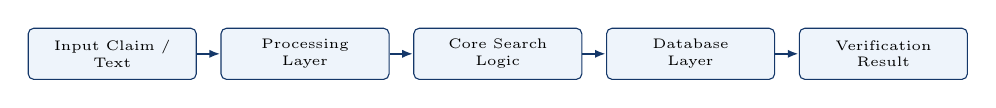
\begin{tikzpicture}[
node distance=3mm,
box/.style={
  rectangle,
  rounded corners=2pt,
  draw=GEUBlue,
  fill=GEULightBlue,
  minimum width=1.90cm,
  minimum height=6.5mm,
  text width=1.90cm,
  align=center,
  font=\tiny
},
arrow/.style={-{Latex[length=1.4mm]},thick,draw=GEUBlue}
]
\node[box] (a) {Input Claim /\\Text};
\node[box,right=of a] (b) {Processing\\Layer};
\node[box,right=of b] (c) {Core Search\\Logic};
\node[box,right=of c] (d) {Database\\Layer};
\node[box,right=of d] (e) {Verification\\Result};
\draw[arrow] (a)--(b);
\draw[arrow] (b)--(c);
\draw[arrow] (c)--(d);
\draw[arrow] (d)--(e);
\end{tikzpicture}
\end{center}

\vspace{0.5mm}
\begin{columns}[T,totalwidth=\textwidth]
\column{.48\textwidth}
\textbf{\color{GEUBlue}\scriptsize Data / Control Flow}
\begin{itemize}\scriptsize\tightlistspacing\RaggedRight
\item User inputs claim or article text for verification.
\item Text is cleaned and keywords are extracted.
\item Hashing and BST search find related stored records.
\item Relevance scoring generates a final classification.
\end{itemize}

\vspace{1mm}
\textbf{\color{GEUBlue}\scriptsize Major System Components}
\begin{itemize}\scriptsize\tightlistspacing\RaggedRight
\item \textbf{Input Module:} Receives raw headline or claim.
\item \textbf{Analyzer Module:} Tokenization and stopword removal.
\item \textbf{Matching Engine:} Compares keywords with database.
\end{itemize}

\column{.48\textwidth}
\textbf{\color{GEUBlue}\scriptsize Processing and Storage Pipeline}
\begin{itemize}\scriptsize\tightlistspacing\RaggedRight
\item \textbf{Input Layer:} Claim text entered by the user.
\item \textbf{Processing Layer:} Validates structure and extracts tokens.
\item \textbf{Core Logic:} Hash lookup, searching, and credibility score.
\item \textbf{Database Layer:} Stores known news and trusted sources.
\item \textbf{Output Layer:} Credibility score and summary status.
\end{itemize}
\end{columns}
\end{frame}

% ============================================================
% 8. TECHNOLOGY STACK AND METHODOLOGY
% ============================================================
\begin{frame}{Technology Stack \& Methodology}
\begin{columns}[T,totalwidth=\textwidth]
\column{.48\textwidth}
\begin{block}{Technology Stack}
\begin{itemize}\scriptsize\tightlistspacing\RaggedRight
\item \textbf{C \& C++}: DSA in C and OOP structuring in C++.
\item \textbf{DSA}: Hashing, BST, searching, and sorting.
\item \textbf{File Handling}: Stores local database and logs.
\item \textbf{VS Code / Code::Blocks}: IDE and build environment.
\item \textbf{Git \& GitHub}: Version control and team tracking.
\end{itemize}
\end{block}

\vspace{1.5mm}
\begin{block}{Purpose}
\scriptsize\RaggedRight
Build a modular, searchable, and explainable news verification prototype.
\end{block}

\column{.48\textwidth}
\begin{block}{Development Methodology}
\begin{enumerate}\scriptsize\tightlistspacing\RaggedRight
\item \textbf{Requirements:} Define parameters, inputs, and outputs.
\item \textbf{Design:} Model classes, hash functions, and trees.
\item \textbf{Implementation:} Build modular C/C++ components.
\item \textbf{Testing:} Verify keyword search with edge cases.
\item \textbf{Evaluation:} Measure score accuracy and latency.
\end{enumerate}
\end{block}
\end{columns}

\vspace{2mm}
\centering\tiny\textbf{Pipeline:} Requirements $\longrightarrow$ Design $\longrightarrow$ Implementation $\longrightarrow$ Testing $\longrightarrow$ Evaluation
\end{frame}

% ============================================================
% 9. INITIAL PROGRESS AND TEAM CONTRIBUTION
% ============================================================
\begin{frame}{Initial Progress \& Team Contribution}
\begin{columns}[T,totalwidth=\textwidth]
\column{.38\textwidth}
\textbf{\color{GEUBlue}\footnotesize Progress Achieved}
\begin{itemize}\scriptsize\tightlistspacing\RaggedRight
\item Problem statement identified
\item Background study completed
\item System requirements drafted
\item Architecture and data flow designed
\item Core DSA concepts mapped
\item Database file schemas established
\item Prototype implementation scheduled
\end{itemize}

\column{.60\textwidth}
\textbf{\color{GEUBlue}\footnotesize Individual Contribution}
\vspace{1mm}
\scriptsize
\renewcommand{\arraystretch}{1.15}
\begin{tabularx}{\linewidth}{@{}>{\RaggedRight\arraybackslash}p{1.75cm}>{\RaggedRight\arraybackslash}p{1.20cm}>{\RaggedRight\arraybackslash}X@{}}
\toprule
Member & Role & Contribution\\
\midrule
Shambhavi Srivastava & Team Lead & Project planning, requirements, and system design coordination\\
Abhinav Panwar & Developer & C++ OOP classes, indexing, and news data management\\
Akshat Sharma & Testing / Docs & Test suite design, verification metrics, and documentation\\
\bottomrule
\end{tabularx}
\end{columns}
\end{frame}

% ============================================================
% 10. ROADMAP, EXPECTED OUTCOMES AND REFERENCES
% ============================================================
\begin{frame}{Roadmap, Expected Outcomes \& References}
\begin{columns}[T,totalwidth=\textwidth]
\column{.50\textwidth}
\textbf{\color{GEUBlue}\footnotesize Roadmap}
\begin{enumerate}\scriptsize\tightlistspacing\RaggedRight
\item \textbf{Phase-I (Analysis \& Design):} Define news schemas, select DSA/OOP structures, and design verification pipeline.
\item \textbf{Phase-II (Development):} Implement modules, hash indexing, matching engine, and file-based data store.
\item \textbf{Phase-III (Testing \& Finalization):} Run structured news test cases, optimize search times, and deliver working tool.
\end{enumerate}

\vspace{1.5mm}
\textbf{\color{GEUBlue}\footnotesize Expected Outcomes}
\begin{itemize}\scriptsize\tightlistspacing\RaggedRight
\item Working TruthCheck preliminary verification engine
\item Sub-second keyword lookups via hashing
\item Transparent, rule-based credibility indicators
\item Foundation for future automated NLP ingestion
\end{itemize}

\column{.46\textwidth}
\textbf{\color{GEUBlue}\footnotesize References}
\begin{enumerate}\scriptsize\tightlistspacing\RaggedRight
\item Data Structures \& Algorithms -- Course Notes
\item Object-Oriented Programming with C++ -- Reference Guide
\item ISO/IEC C++ Standard Documentation
\item GitHub Repository for Team Version Tracking
\end{enumerate}

\vspace{4mm}
\begingroup
\centering
\noindent\colorbox{GEUBlue}{%
\parbox{\dimexpr\linewidth-2\fboxsep\relax}{%
\centering\vspace{2mm}%
\color{white}\textbf{\small Thank You}\\[1mm]
\scriptsize Questions \& Suggestions
\vspace{2mm}%
}}%
\par
\endgroup
\end{columns}
\end{frame}

\end{document}